\documentclass[10pt,twocolumn]{article}

% use the oxycomps style file
\usepackage{oxycomps}

% usage: \fixme[comments describing issue]{text to be fixed}
% define \fixme as not doing anything special
\newcommand{\fixme}[2][]{#2}
% overwrite it so it shows up as red
\renewcommand{\fixme}[2][]{\textcolor{red}{#2}}
% overwrite it again so related text shows as footnotes
%\renewcommand{\fixme}[2][]{\textcolor{red}{#2\footnote{#1}}}

% read references.bib for the bibtex data
\bibliography{references}

% include metadata in the generated pdf file
\pdfinfo{
    /Title (The Occidental Computer Science Comprehensive Project: Goals, Timeline, Format, and Advice)
    /Author (Justin Li)
}

% set the title and author information
\title{Git Tutorial - Junior Seminar}
\author{Luis Martinez}
\affiliation{Occidental College}
\email{lmartinez3@oxy.edu}

\begin{document}

\maketitle

\section{What is Git:}

Git is a distributed version control system that records changes in files, allowing access to specific versions of those files at any given time. It facilitates collaborative work by enabling individuals to work on copies of a project before syncing them. Additionally, it syncs with GitHub.

\section{Installing Git:}

To install Git, download it from the Git website (git-scm.com). It also serves as a reference website. For Windows users, there is an option to use the command line. After installation, verify by opening your terminal and entering: \texttt{git --version}.

\section{GitHub:}

GitHub is the most popular and free-to-use remote repository platform. Users can create a GitHub account, host repositories, and share and discover other users' repositories.

\subsection{Tip:}

Create a folder to store all of your local repositories.

\section{For this tutorial we'll be using GitKraken:}

\begin{figure}[htbp]
\centering
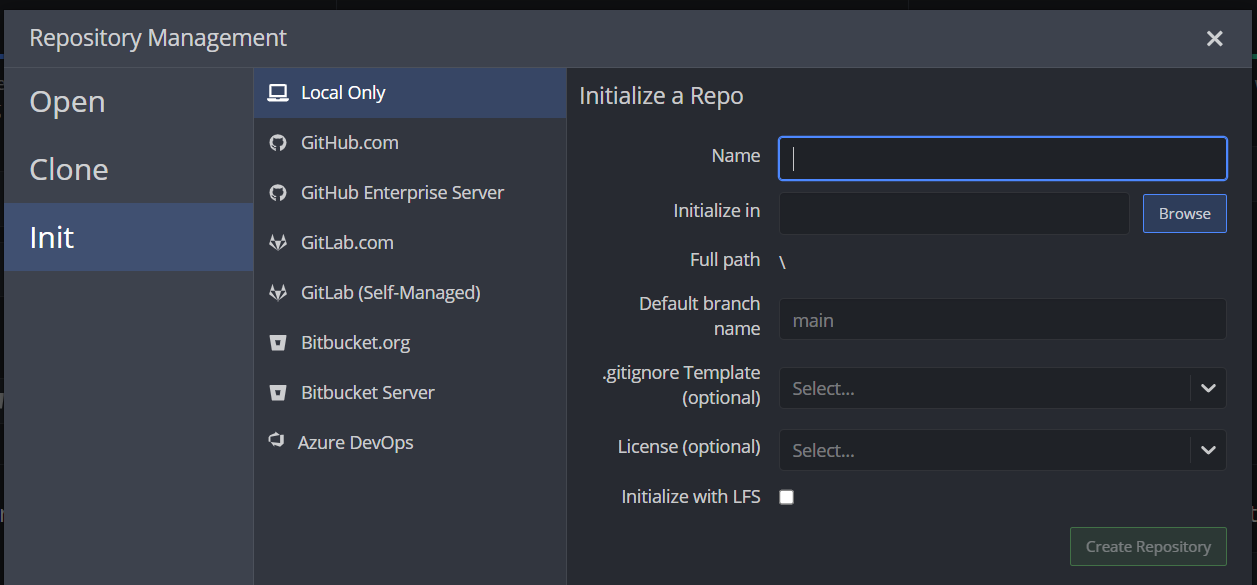
\includegraphics[width=0.5\textwidth]{First Pic.png}
\label{fig:my_label}
\end{figure}

After installing GitKraken, open the application and log in using your GitHub account. Upon logging in, you'll see the option to get started, where you can select "Create repo". You can also connect your GitHub account with GitKraken. Create a "Local Only" Repo named "Learn-Gitkraken" and select the folder to initialize the repo. Then, click "Create Repository". You'll now see your repo with a README file in your computer's library.


\section{Next we'll add a file to the repo:}

In the repo folder, add a new text file named "text\_for\_git.txt". In GitKraken, you'll notice a file change in the working directory. Click on "view change". This will bring up the staged and unstaged files. You will see that our text file is under the Unstaged Files section. Click on the "Stage all Files Button".

\begin{figure}[htbp]
\centering
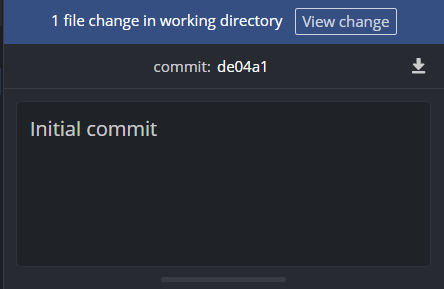
\includegraphics[width=0.5\textwidth]{second.png}
\label{fig:my_label}
\end{figure}

\section{What is Staging and Committing:}

In git, we keep a history of commits. They're kind of like save points for code that you can revert to at your choosing. Notably, this works with an entire project, not just individual files. The files that you want to be part of your commit first go on the git index which is "staging" them. You can also put in a commit message, let's say "first commit". Then click "Commit Changes". You will then see on GitKraken's UI that there is a change in the commit history.

\begin{figure}[htbp]
\centering
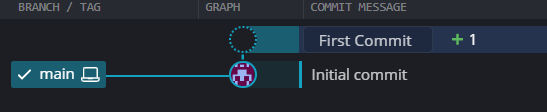
\includegraphics[width=0.5\textwidth]{fourth.png}
\label{fig:my_label}
\end{figure}

\section{Let's Try adding another File:}

Let's call it second.text. It is automatically added to our unstaged file section. Stage it and commit it. Let's add a third file called "third" and stage and commit it. Your GitKraken should now look like this.

\begin{figure}[htbp]
\centering
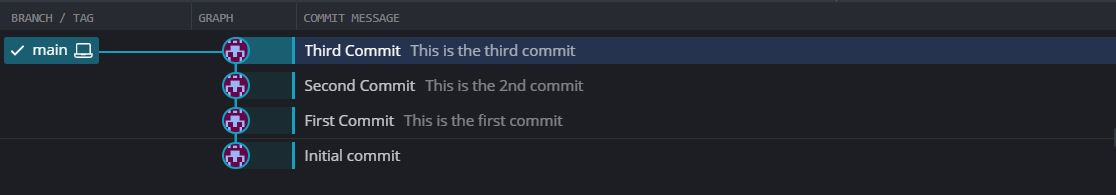
\includegraphics[width=0.5\textwidth]{fifth.png}
\label{fig:my_label}
\end{figure}

\section{Revert Commit:}

Let's say we want to go back to a version of our folder without "second.txt". Right-click on "Second Commit" which will bring up a menu and select "Reverse commit". GitKraken will ask you to confirm if you want to revert. Select Yes. This will remove the file from your folder and show a new commit in your history called "Revert Second Commit" as seen below.

\begin{figure}[htbp]
\centering
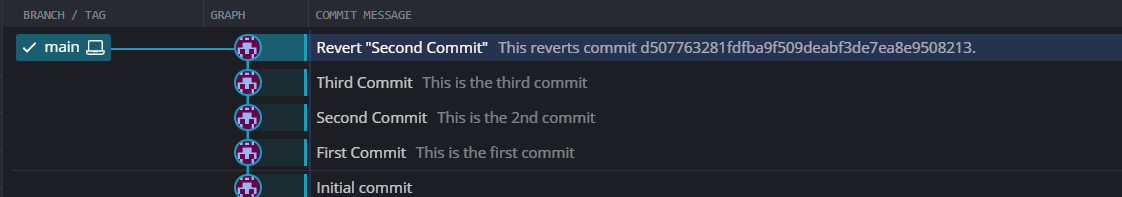
\includegraphics[width=0.5\textwidth]{sixth.png}
\label{fig:my_label}
\end{figure}

\section{In addition to Revert Commit you can also Rest Commit in order to manipulate your commit history, but what is the difference between them?}

Start by adding a new file called "fourth.txt" and stage and commit it. Add a fifth file called "fifth.txt" and stage and commit it. Your commit history should look like the below image… Right-click on the second commit. In the menu click reset main to this commit and scroll down to "Hard - discard all changes". This will revert and remove all of the changes after "Second Commit" and it will bring back the "second.txt" file.
\begin{figure}[htbp]
\centering
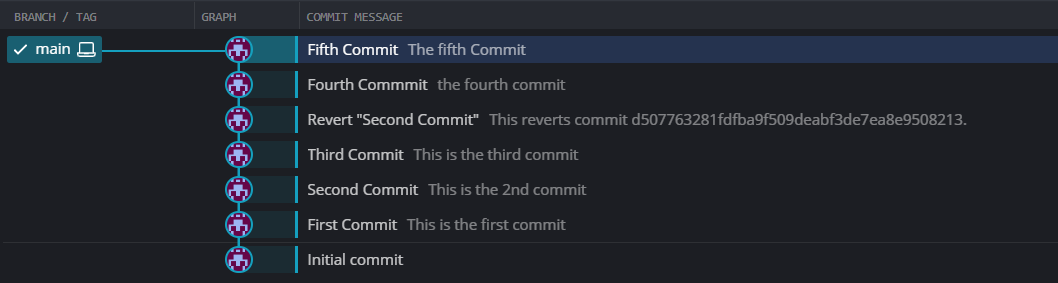
\includegraphics[width=0.5\textwidth]{seven.png}
\label{fig:my_label}
\end{figure}
\begin{figure}[htbp]
\centering
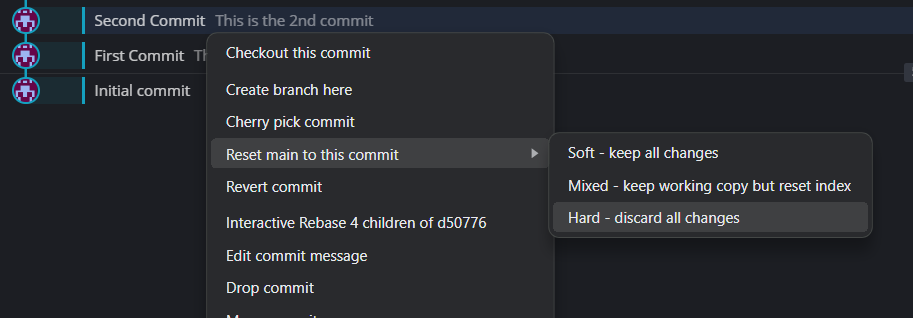
\includegraphics[width=0.5\textwidth]{eight.png}
\label{fig:my_label}
\end{figure}

\section{Tagging:}

You can also add tags to the Branch or a Commit by right-clicking it and scrolling down. They serve as a way of marking down an important part of your project and making it easily searchable by looking at the "Tags".

\begin{figure}[htbp]
\centering

\includegraphics[width=0.5\textwidth]{nine.png}
\label{fig:my_label}
\end{figure}

\section{Branching:}

Branches give coders the ability to work in an isolated version of the code that allows them to work without affecting the overall project. If the work they do is good and works, they can then merge their work into the original code or the "Main" branch. If they did a bad job, they can simply delete the branch with no negative effects. To create a new branch, right-click on the "main" branch and select "create branch here". Let's name this branch "secondary". Your GitKraken should now look something like this. Let's create two more branches called "tertiary" and "quaternary". Make sure you're in the main branch. In your repository's folder, create a new text filed called "hello\_world" and type "Hello World" into it then save. Stage and commit this file.

\begin{figure}[htbp]
\centering
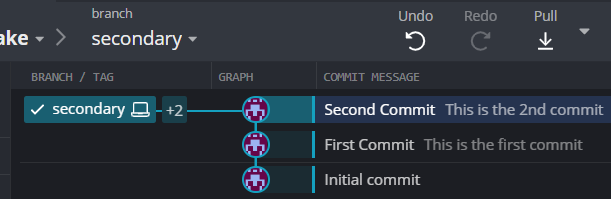
\includegraphics[width=0.5\textwidth]{ten.png}
\label{fig:my_label}
\end{figure}


Switch to the "secondary" branch. You'll notice that if you look at your folder while on the secondary branch you cannot access the "hello\_world" file. Create a new text file (let's call it hello\_again) and fill it with some text, let's say "Hello my baby, Hello my Honey". Stage and commit the file. Your GitKraken should now look something like this. Let's add another text file to the Secondary Branch. Stage and Commit it. GitKraken should look something like this.

\begin{figure}[htbp]
\centering
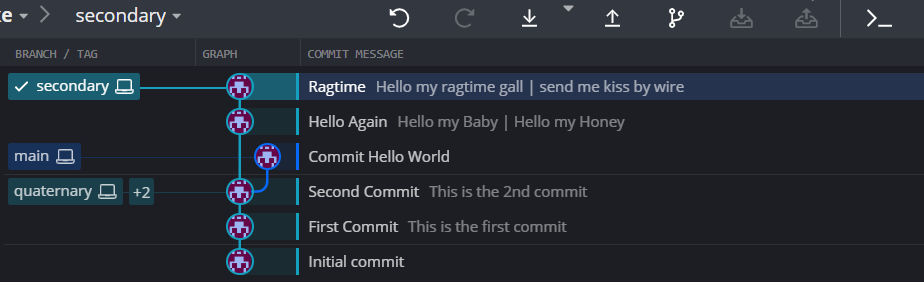
\includegraphics[width=0.5\textwidth]{11.png}
\label{fig:my_label}
\end{figure}

\section{Let's Merge secondary into main:}

Select/enter the main branch. right-click on secondary and select "Merge secondary into main". Your gitkraken should now look something like this. Now the text files from secondary AND main are in the main branch of the repository.

\begin{figure}[htbp]
\centering
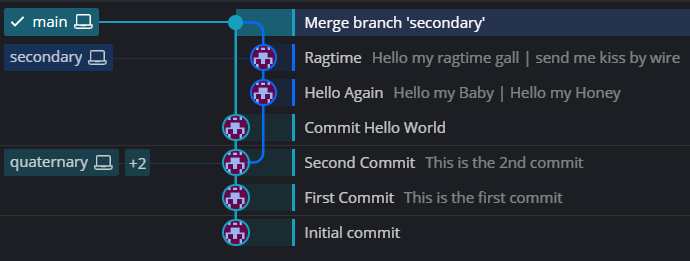
\includegraphics[width=0.5\textwidth]{12.png}
\label{fig:my_label}
\end{figure}

\section{Select the tertiary branch}

Create a text file and commit it. You can also branch off a branch the same way you branched off of main. Right-click the tertiary branch and create a new branch. I called this branch of tertiary "tertiary\_sequel". Add a text file to your new branch and commit it. Add and commit another text file. Your gitkraken should look something like this.

\begin{figure}[htbp]
\centering
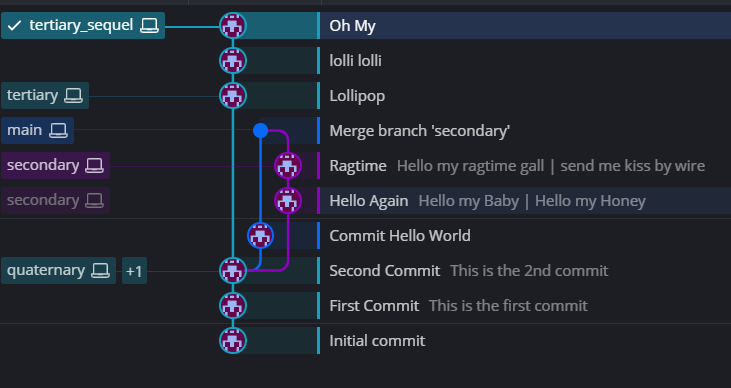
\includegraphics[width=0.5\textwidth]{13.png}
\label{fig:my_label}
\end{figure}

\section{Switch to the Quaternary Branch}

Right Click on your latest commit in "tertiary\_sequel" and select "Cherry pick commit". This allows you to only merge changes from a single commit rather than an entire branch. Your git kraken should now look something like this.

\begin{figure}[htbp]
\centering
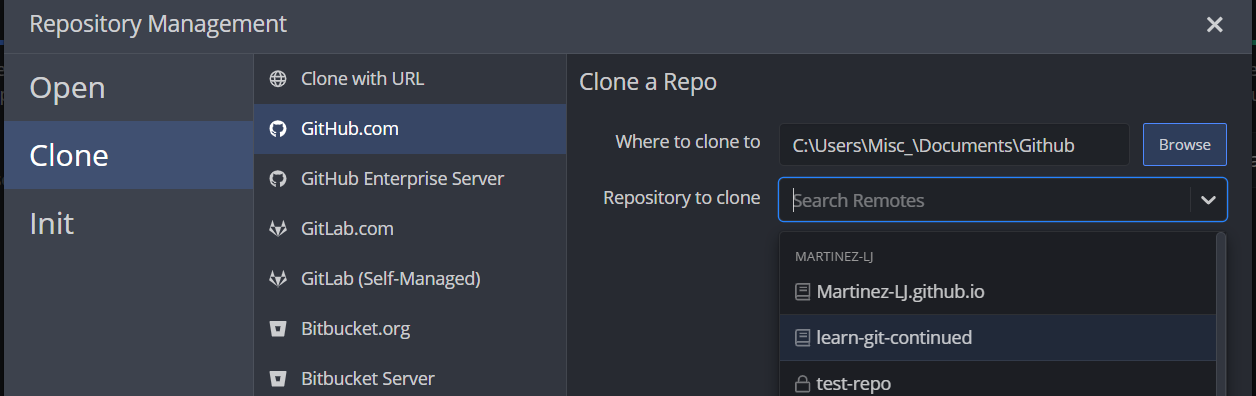
\includegraphics[width=0.5\textwidth]{14.png}
\label{fig:my_label}
\end{figure}

\section{Now let's merge everything into main}

Your GitKraken should now look something like this. You can also delete branches by right-clicking and selecting "Delete 'Branch Name' ".

\begin{figure}[htbp]
\centering
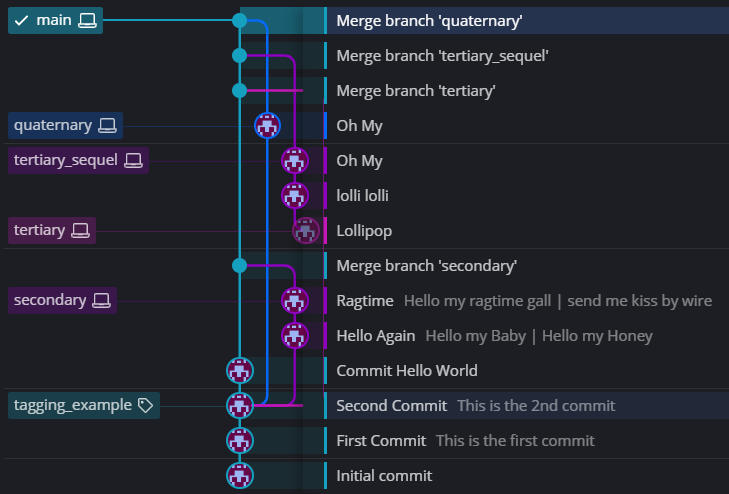
\includegraphics[width=0.5\textwidth]{15.png}
\label{fig:my_label}
\end{figure}

\section{Merging Conflicts:}

Merging conflicts happen when more than one person works on the same file on different branches and tries to merge them to the same branch. The best way to fix it is to avoid it by having good communication, but let's see how you fix it when it occurs. Let's say you have a merge conflict with a text file. Open the file, it will show the differences between both files and you'll have to edit it manually to see what you want to actually keep and commit. Now commit and merge as normal.

\section{Let's look at cloning Github Repositories:}

Click on File or the File Icon and select Clone or Clone repo. Here you have the option to Clone based off a URL or, if you select the Github.com tab, you have the option to clone a repository from your Github account. For the purpose of this tutorial, I created an empty repository on Github.com called learn-git-continued. I left it public and clicked the box to add a README file. Now clone the repo you want from Github. Now let's add text file into the cloned repo in the folder you cloned the repo into. Let's call it "hello\_again.txt". Stage and commit it. If you look at your repo in Github, you will notice that it doesn't have the commit we just made. To get the change from your local machine to Github, you have to Push it to your Github. Click the Push button. If you look at your Github you will see that it now has the file. If you don't see it, refresh your page.

\section{Let's Try adding a file from our Github to our local machine:}

Let's call it git\_hello and commit changes. To sync this change to your local machine, click on the Pull Button. You should now see that the file from your Github (your remote repo) has been added to your local machine on GitKraken.

\section{Pull Requests:}

To help manage the project, people will use something called Pull Request to get files from the remote repository. Essentially, you're asking permission to access the files. Add a new file to your remote repo, let's call it "pull\_practice". To make a Pull Request, hover over the Pull Request menu and click on the green plus button. The following menu will be brought up. Select the repo you want to pull from and where you want it as well as the branch you want to pull from and commit to. Finally, add a title and click "create pull request". You will then see on Github that you have received a notification for a Pull Request and can choose to allow it or deny it.

\printbibliography

\end{document}
